\documentclass{article}

\usepackage[a4paper]{geometry}
\usepackage[ngerman]{babel}
\usepackage[utf8]{inputenc}
\usepackage[T1]{fontenc}
\usepackage{graphicx}
\usepackage{fancyhdr}
\usepackage{xcolor}
\usepackage{float}
\usepackage{hyperref}

\graphicspath{{./images/}}

\pagestyle{fancyplain}
\fancyhf{}
\lhead{\fancyplain{}{Gruppe 11 – Mathias Baumbach \& Mara Schulke} }
\rhead{\fancyplain{}{\today}}
\cfoot{\fancyplain{}{\thepage}}

\begin{document}

\begin{titlepage}
	\begin{flushleft}
		TH Brandenburg \\
		Online Studiengang IT Sicherheit \\
		Fachbereich Informatik und Medien \\
		Netzwerksicherheit \\
		Prof.\ Dr.\ Michael Pilgermann
	\end{flushleft}

	\vfill

	\begin{center}
		\Large{Einsendeaufgabe 1}\\[0.5em]
		\large{Wintersemester 2023}\\[0.25em]
		\large{Abgabetermin \today}
	\end{center}

	\vfill

	\begin{flushright}
		Gruppe 11 \\
		Mathias Baumbach (Matr-Nr. 20213703) \\
		Mara Schulke (Matr-Nr. 20215853)
	\end{flushright}
\end{titlepage}

\begin{abstract}
	Innerhalb dieser Einsendeaufgabe werden verschiedene Aspekte der Netzwerksicherheit – vor 
	allem aus der Angreiferperspektive – betrachtet. Im Rahmen der Bearbeitung konnten wir 
	wertvolle Erfahrungen sammeln – gerade die Aufgabe 2.5 (Google-Hacking) hat uns erneut vor 
	Augen geführt wie wichtig eine entsprechende Absicherung von IT-Systemen ist, da wir 
	innerhalb von wenigen Minuten vollen Zugriff auf die Datenbank eines PHP Web-Servers 
	erlangen konnten. Wir haben den Betreiber informiert und anonymisiert. So, dass diese 
	Dokumentation nicht zu einer weiteren Ausnutzung verwendet werden kann.
\end{abstract}

\tableofcontents

\listoffigures

\newpage

\section{Vorbereitungen}

Die bevorzugte Methode zur Beantwortung der Einsendeaufgabe besteht darin, dass Sie 
entweder ParrotOS oder Kali Linux als virtuelle Maschine auf Ihrem Rechner installieren. 
Diese beiden Linux-Distributionen sind speziell auf die IT-Sicherheit ausgelegt und haben 
daher viele interessante Tools schon vorinstalliert. 
Tipp zur Durchführung: Laden Sie von ParrotOS  eine .ova für virtuelle Maschinen herunter 
(genauer die .ova der Security Edition; Tipp: das Superuser-Password lautet dann "parrot" 
und nicht "toor" wie bei anderen Versionen). Falls noch nicht vorhanden, installieren Sie 
Virtualbox  und führen die virtuelle Maschine darin aus.
Leider gibt es in der letzten Zeit zunehmend Prozessorarchitekturen (gerade für Mac), bei 
denen keine Möglichkeit zum Betrieb von virtuellen Maschinen besteht. Sollte das der Fall 
sein, dann bearbeiten Sie die Aufgaben auf Ihrem eigenen Betriebssystem. Sie müssen dafür 
die Tools einzeln herunterladen.

\newpage

\section{Durchführung}

\subsection{Telnet und Wireshark}

\subsubsection*{Aufgabenstellung}

Wireshark ist bei ParrotOS und Kali Linux vorinstalliert. Es kann ansonsten von der 
Wireshark-Seite heruntergeladen werden. In der Wireshark-Datei im Kurs (telnet.pcapng) ist 
eine Aufzeichnung eines Einlog-Vorgangs mit Telnet zu finden. Suchen Sie darin das 
Passwort.

\subsubsection*{Antwort}

Nach dem wir die Datei analysiert und den Telnet-Login-Vorgang bei dem Paket 
\textcolor{red}{XY} lokalisiert haben, konnten wir den Start des Passwords in Text-Form 
bei dem Paket \textcolor{red}{YZ} entdeckend. (Siehe Abb. 1).

\begin{figure}[H]
	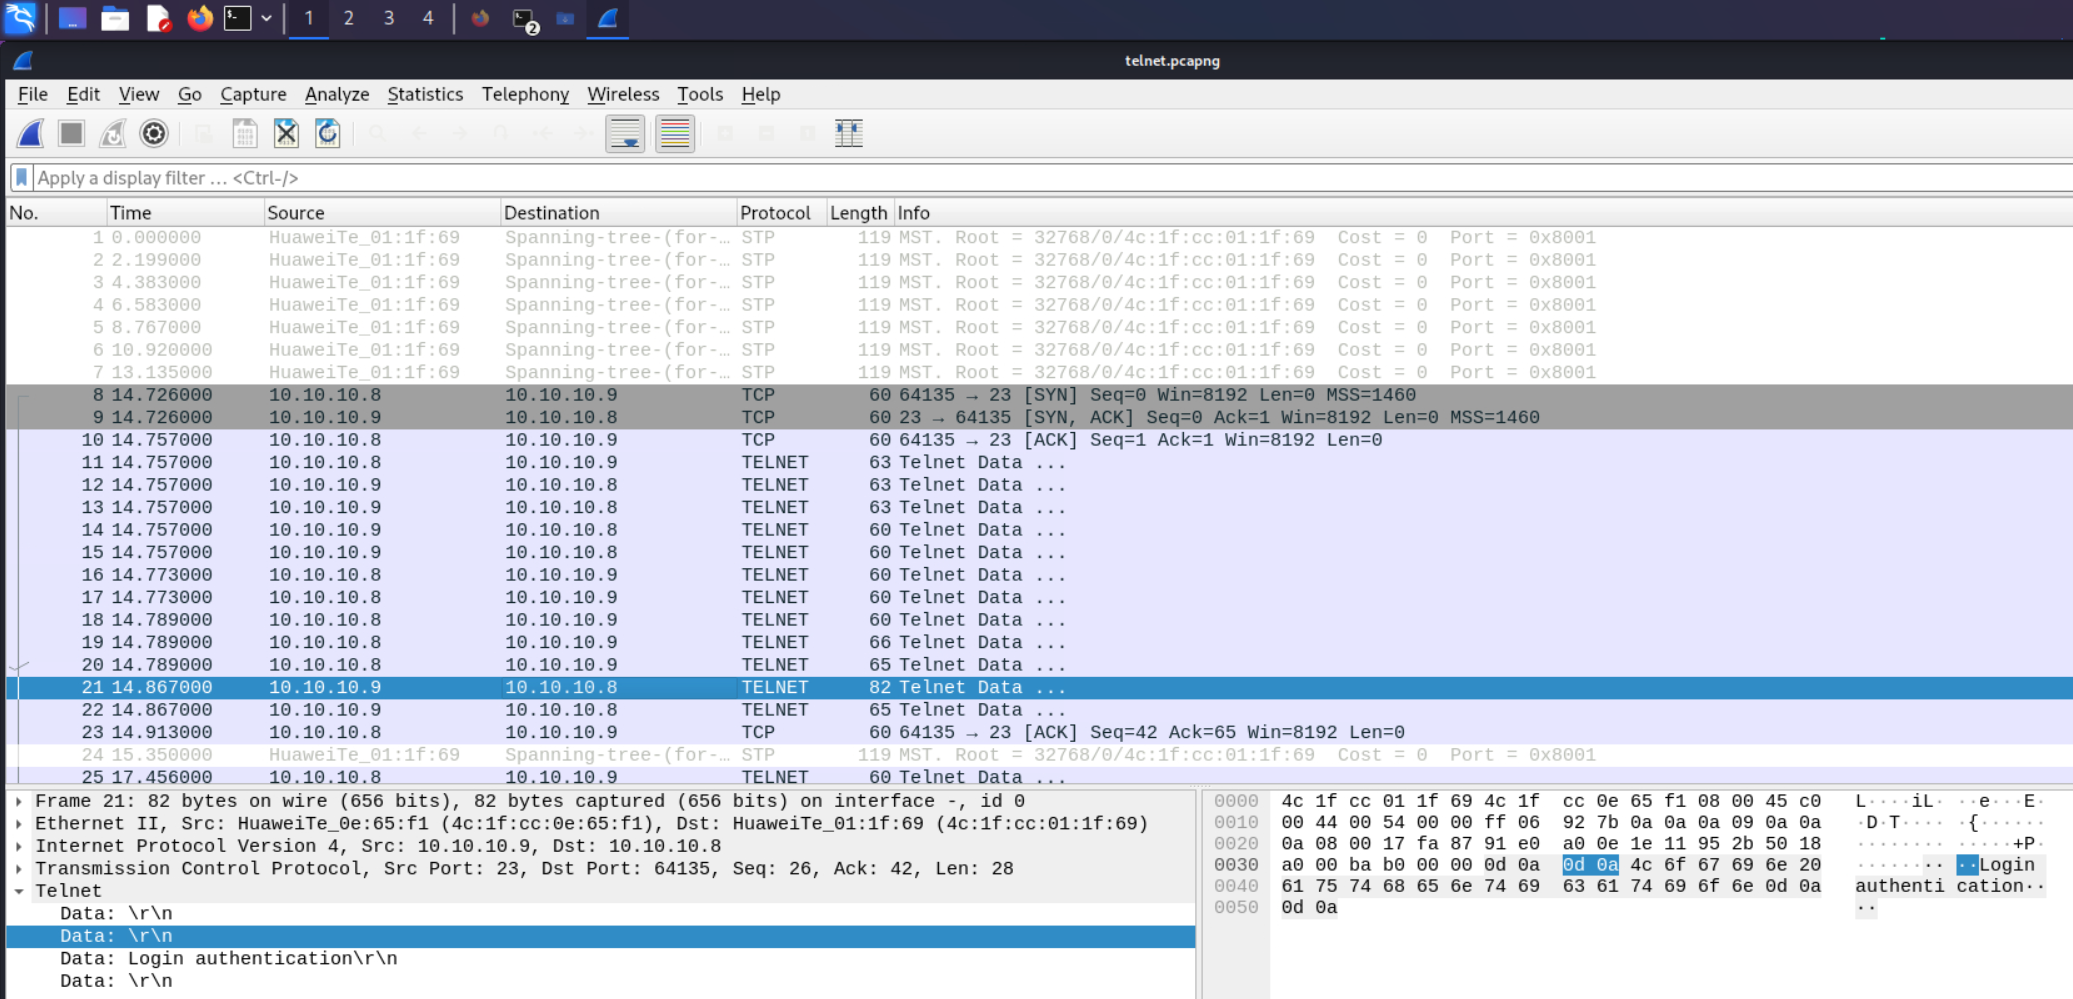
\includegraphics[width=0.75\textwidth]{images/01}
	\centering
	\caption{Telnet Datei: Start des Logins}
\end{figure}

Nun enthielt jedes weitere Paket ein Zeichen des Passworts, bis die End-Sequenz
in dem Paket \textcolor{red}{YY} gesendet wurde. Zusammengesetzt ergibt dies das 
Passwort \texttt{sshnutzen}. (Siehe Abb. 2).

\begin{figure}[H]
	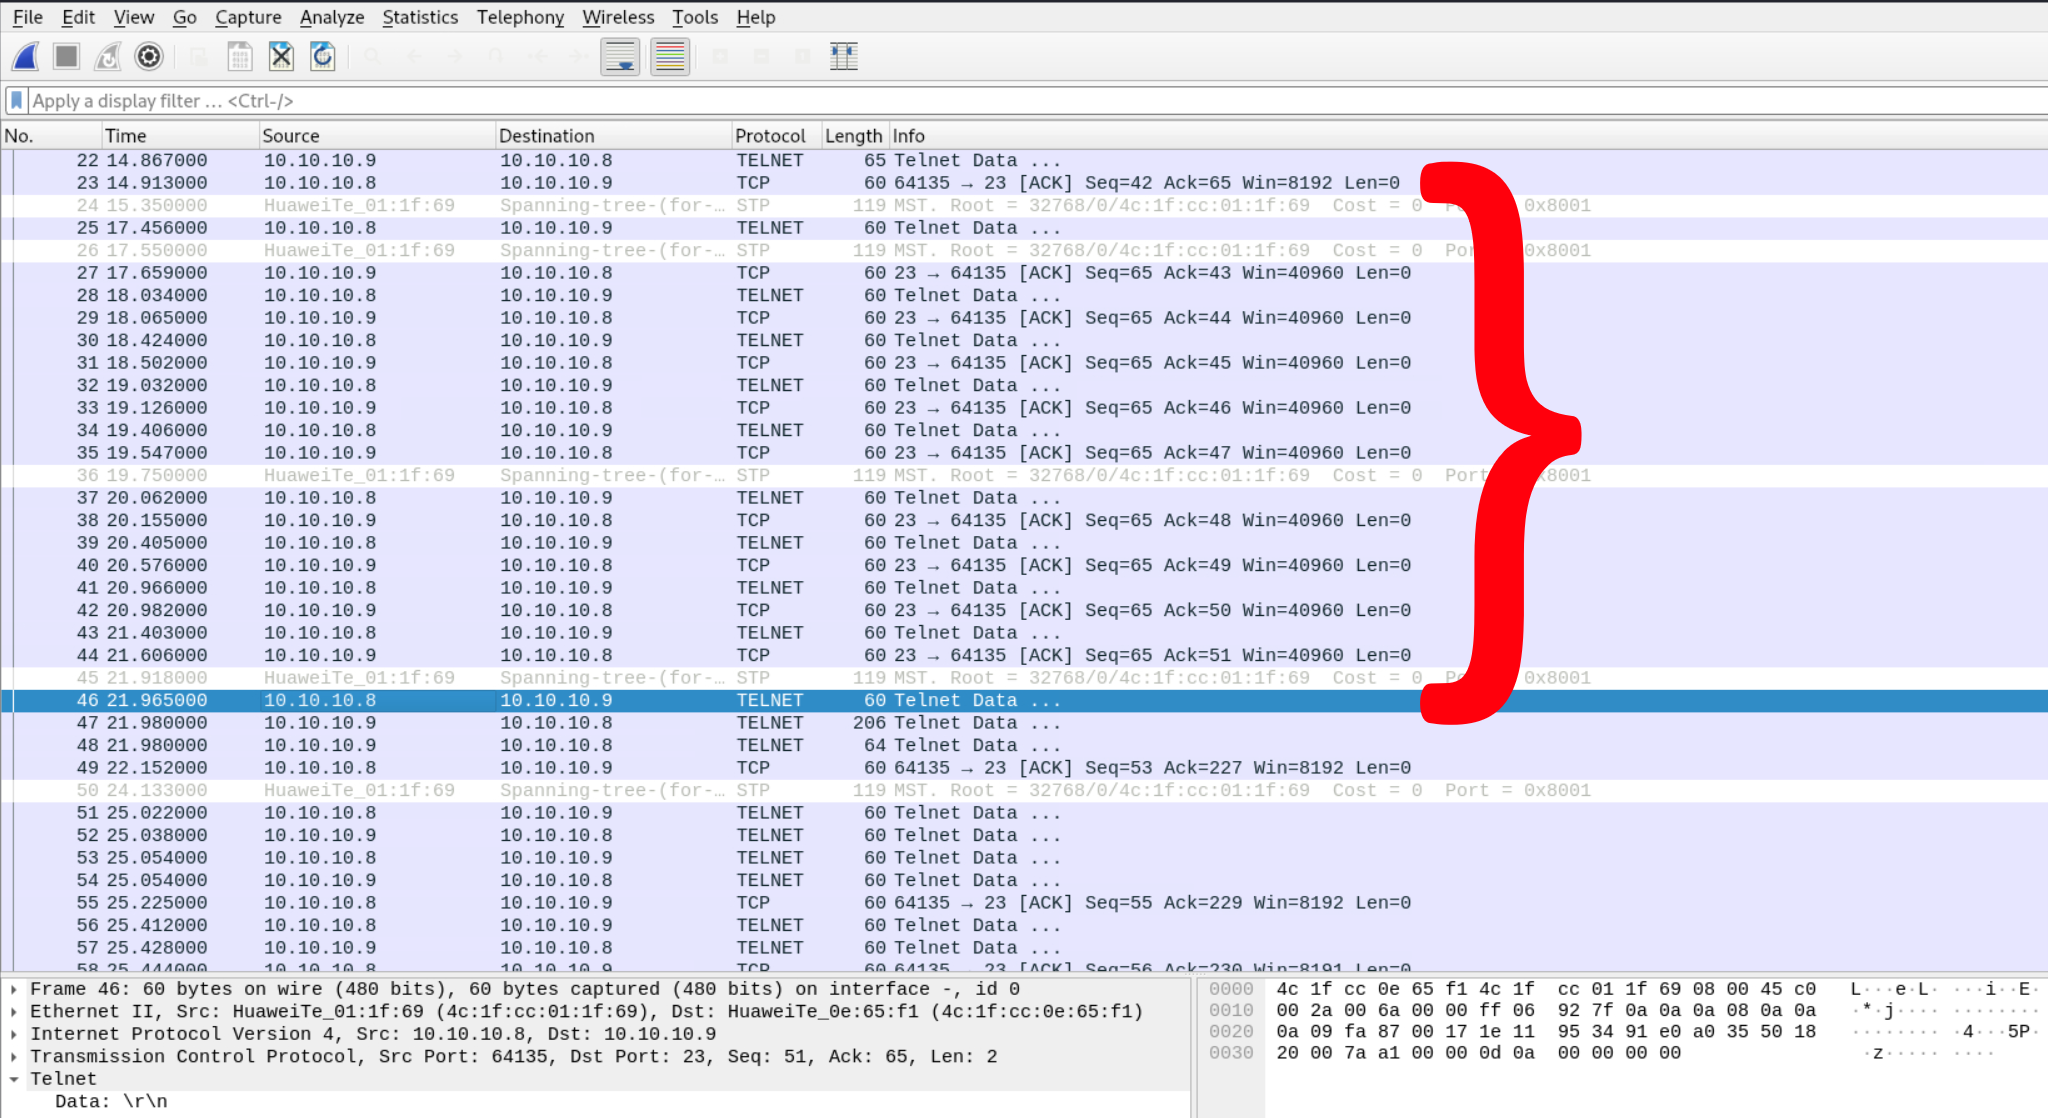
\includegraphics[width=0.75\textwidth]{images/02}
	\centering
	\caption{Telnet Datei: Login Sequenz Dauer}
\end{figure}

\newpage

\subsection{Schwachstellenscan I}

\subsubsection*{Aufgabenstellung}

Verwenden Sie \texttt{nmap} (bei ParrotOS und Kali Linux vorinstalliert), um verschiedene 
Scans des Testservers nwsmooc.mooin.org durchzuführen. Erklären Sie die Ergebnisse, wobei 
mindestens drei Tests mit jeweils unterschiedlichen Parametern durchgeführt werden müssen. 
Versuchen Sie dabei u.a. herauszufinden, welche Dienste auf dem Zielserver installiert
sind und welches Betriebssystem verwendet wird.

\subsubsection*{Antwort}

Der Aufgabe entsprechend haben wir drei sinnvolle \texttt{nmap} scans durchgeführt. 

\begin{figure}[H]
	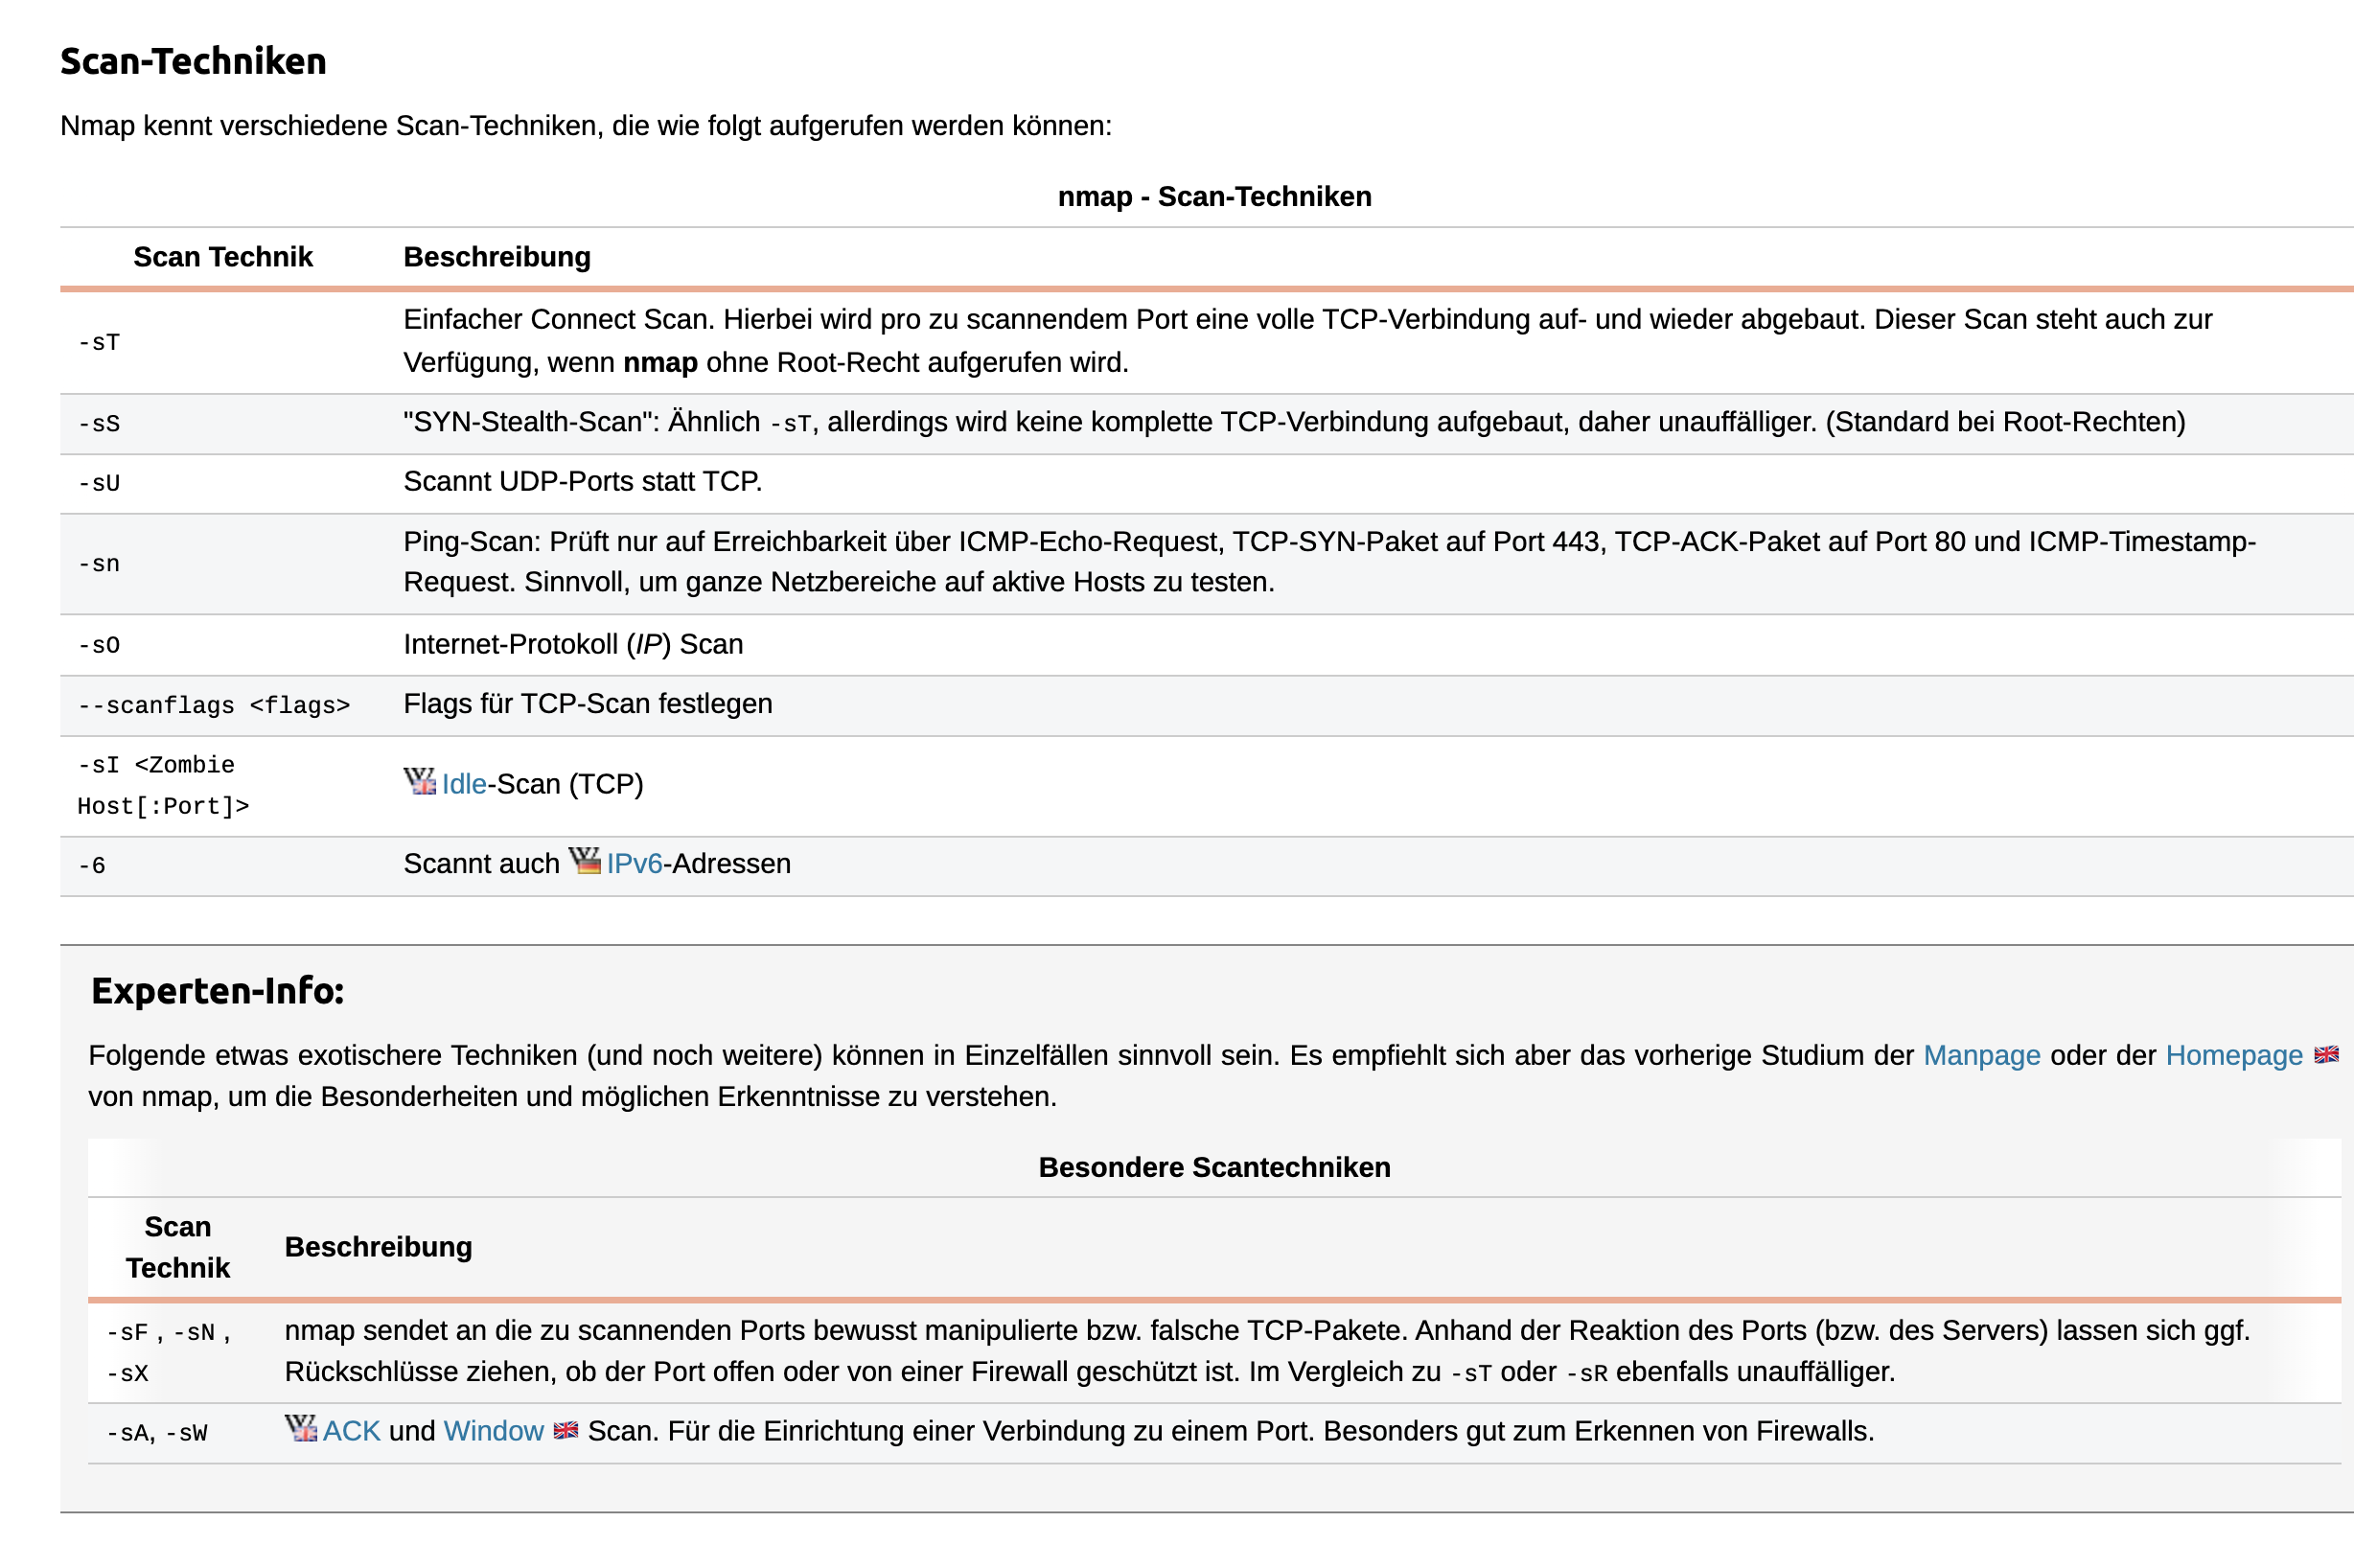
\includegraphics[width=0.75\textwidth]{images/03}
	\centering
	\caption{nmap: Scan-Techniken}
\end{figure}

\subsubsection*{Port Scan}

\begin{figure}[H]
	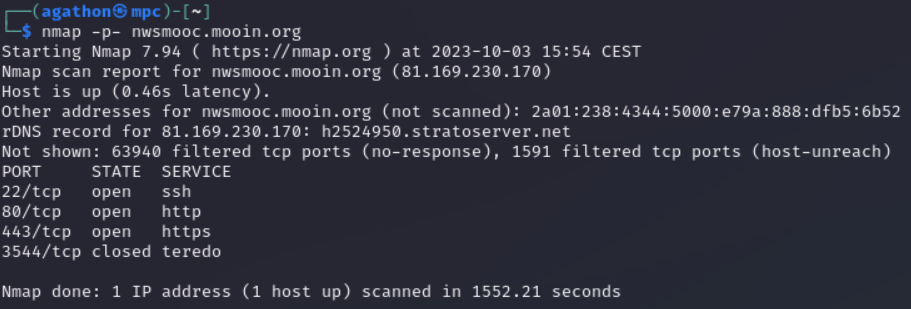
\includegraphics[width=0.75\textwidth]{images/04}
	\centering
	\caption{nmap: Port Scan}
\end{figure}

\subsubsection*{TCP Scan}

\begin{figure}[H]
	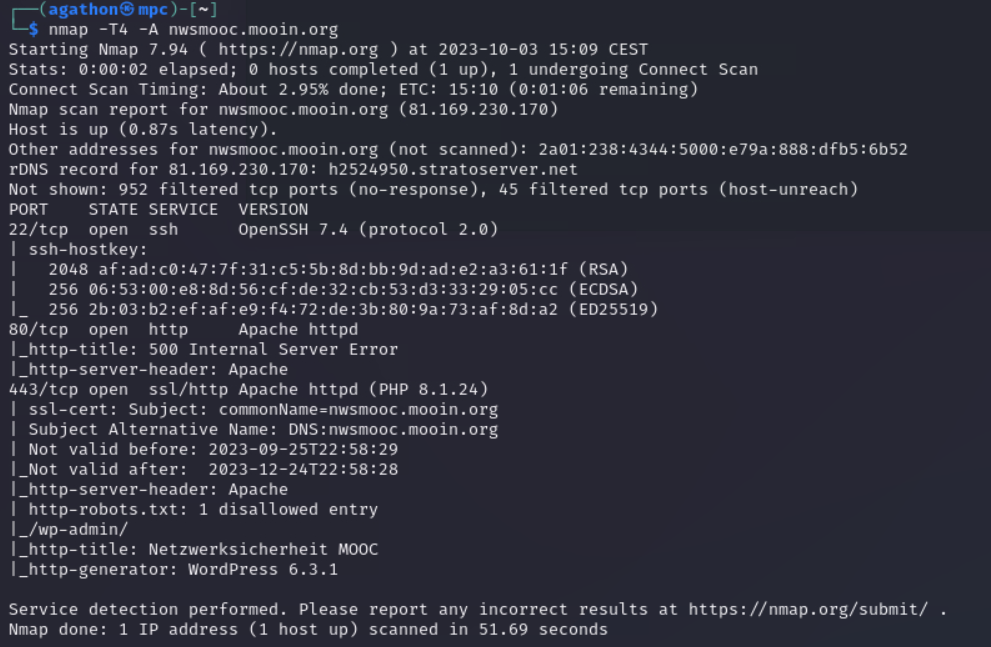
\includegraphics[width=0.75\textwidth]{images/05}
	\centering
	\caption{nmap: TCP Scan}
\end{figure}

\subsubsection*{OS Scan}

\begin{figure}[H]
	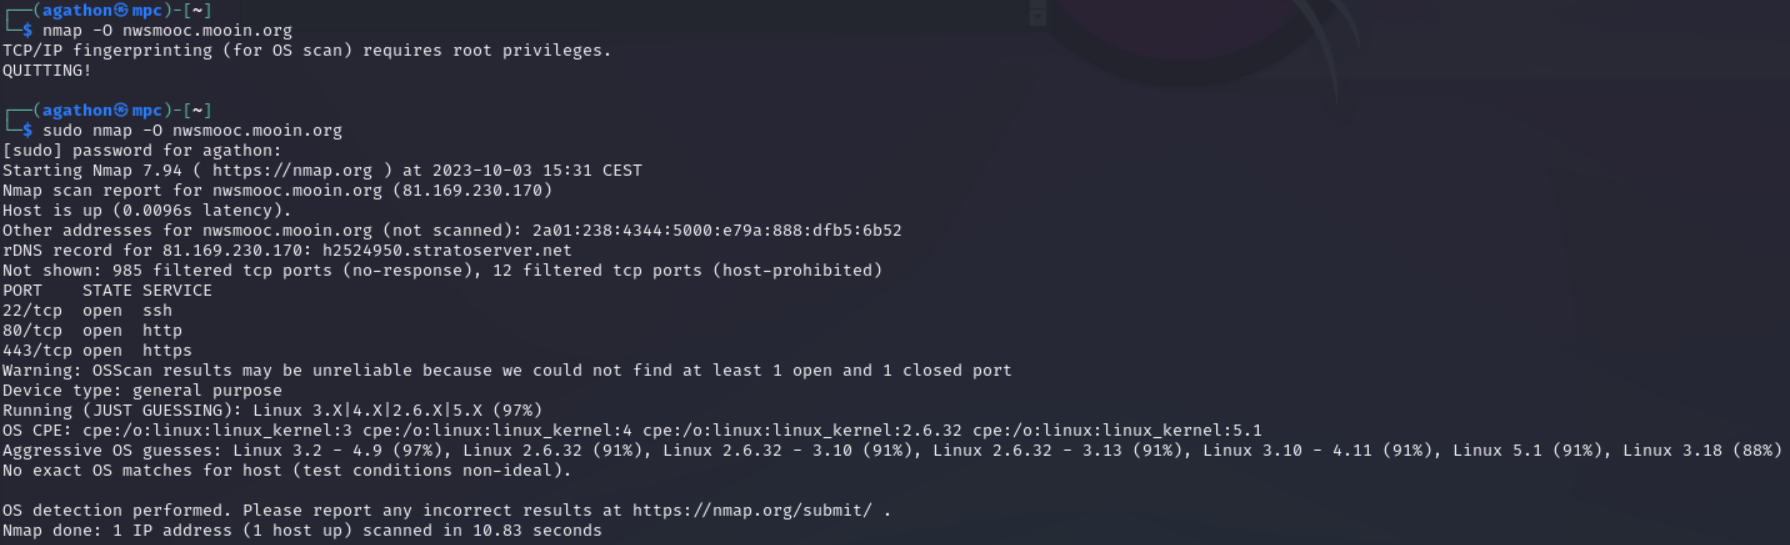
\includegraphics[width=0.75\textwidth]{images/06}
	\centering
	\caption{nmap: OS Scan}
\end{figure}

\subsubsection*{UDP Scan}

\begin{figure}[H]
	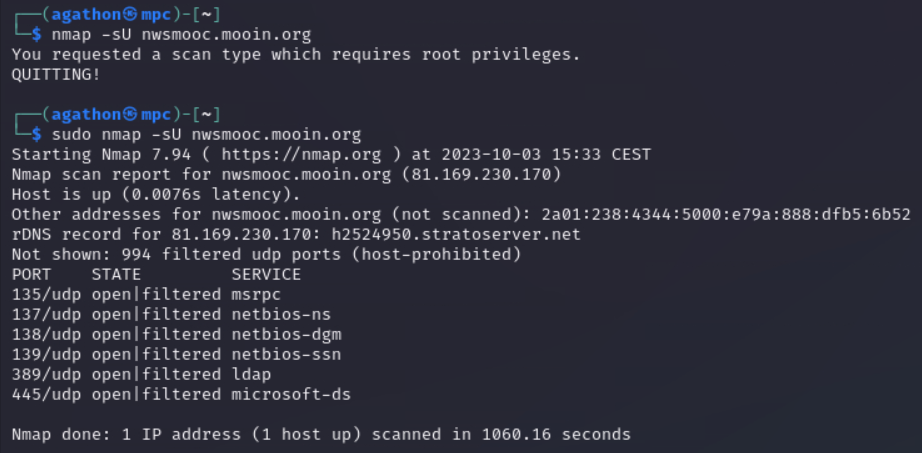
\includegraphics[width=0.75\textwidth]{images/07}
	\centering
	\caption{nmap: UDP Scan}
\end{figure}

\newpage

\subsection{MAC Spoofing}

\subsubsection*{Aufgabenstellung}

Ebenfalls bereits bei ParrotOS und Kali schon vorinstalliert ist das Tool 
\texttt{macchanger}. Machen Sie sich mit dessen Möglichkeiten vertraut, wobei z.B. ein 
Video von HackerSploit nützlich sein kann: \url{https://www.youtube.com/watch?v=bshXz5r-CQA.}
Senden Sie anschließend Datenverkehr mit gefälschter MAC-Adresse und zeichnen diesen mit 
Wireshark auf. Fertigen Sie geeignete Screenshots mit Erklärungen (wie müsste es richtig 
sein? wo ist die gefälschte MAC-Adresse in Wireshark zu sehen?) dazu an.
Mac- und Linux-Nutzer verwenden für die Aufgabe ebenfalls \texttt{macchanger} oder 
\texttt{ifconfig}. Windows-Nutzer schauen sich bitte das Youtube-Tutorial an:
\url{https://www.youtube.com/watch?v=V3Pcc8b_m0U.}
Hinweis: Bei der ersten Methode heißt der Eintrag in den erweiterten Einstellungen nicht
"Network Address", sondern "Locally Administered Address".

\subsubsection*{Antwort}

Um die MAC-Adresse unter Kali-Linux zu ändern genügte eine einfache Kombination aus dem 
Programm \texttt{macchanger} und \texttt{ifconfig}. Zu erst, um eine erfolgreiche Änderung 
bzw. ein erfolgreiches Spoofing feststellen zu können, haben wir den Netzwerk-Verkehr zum 
Web-Server der vorherigen Aufgaben wiederverwendet. (Siehe Abb. X)

\begin{figure}[H]
	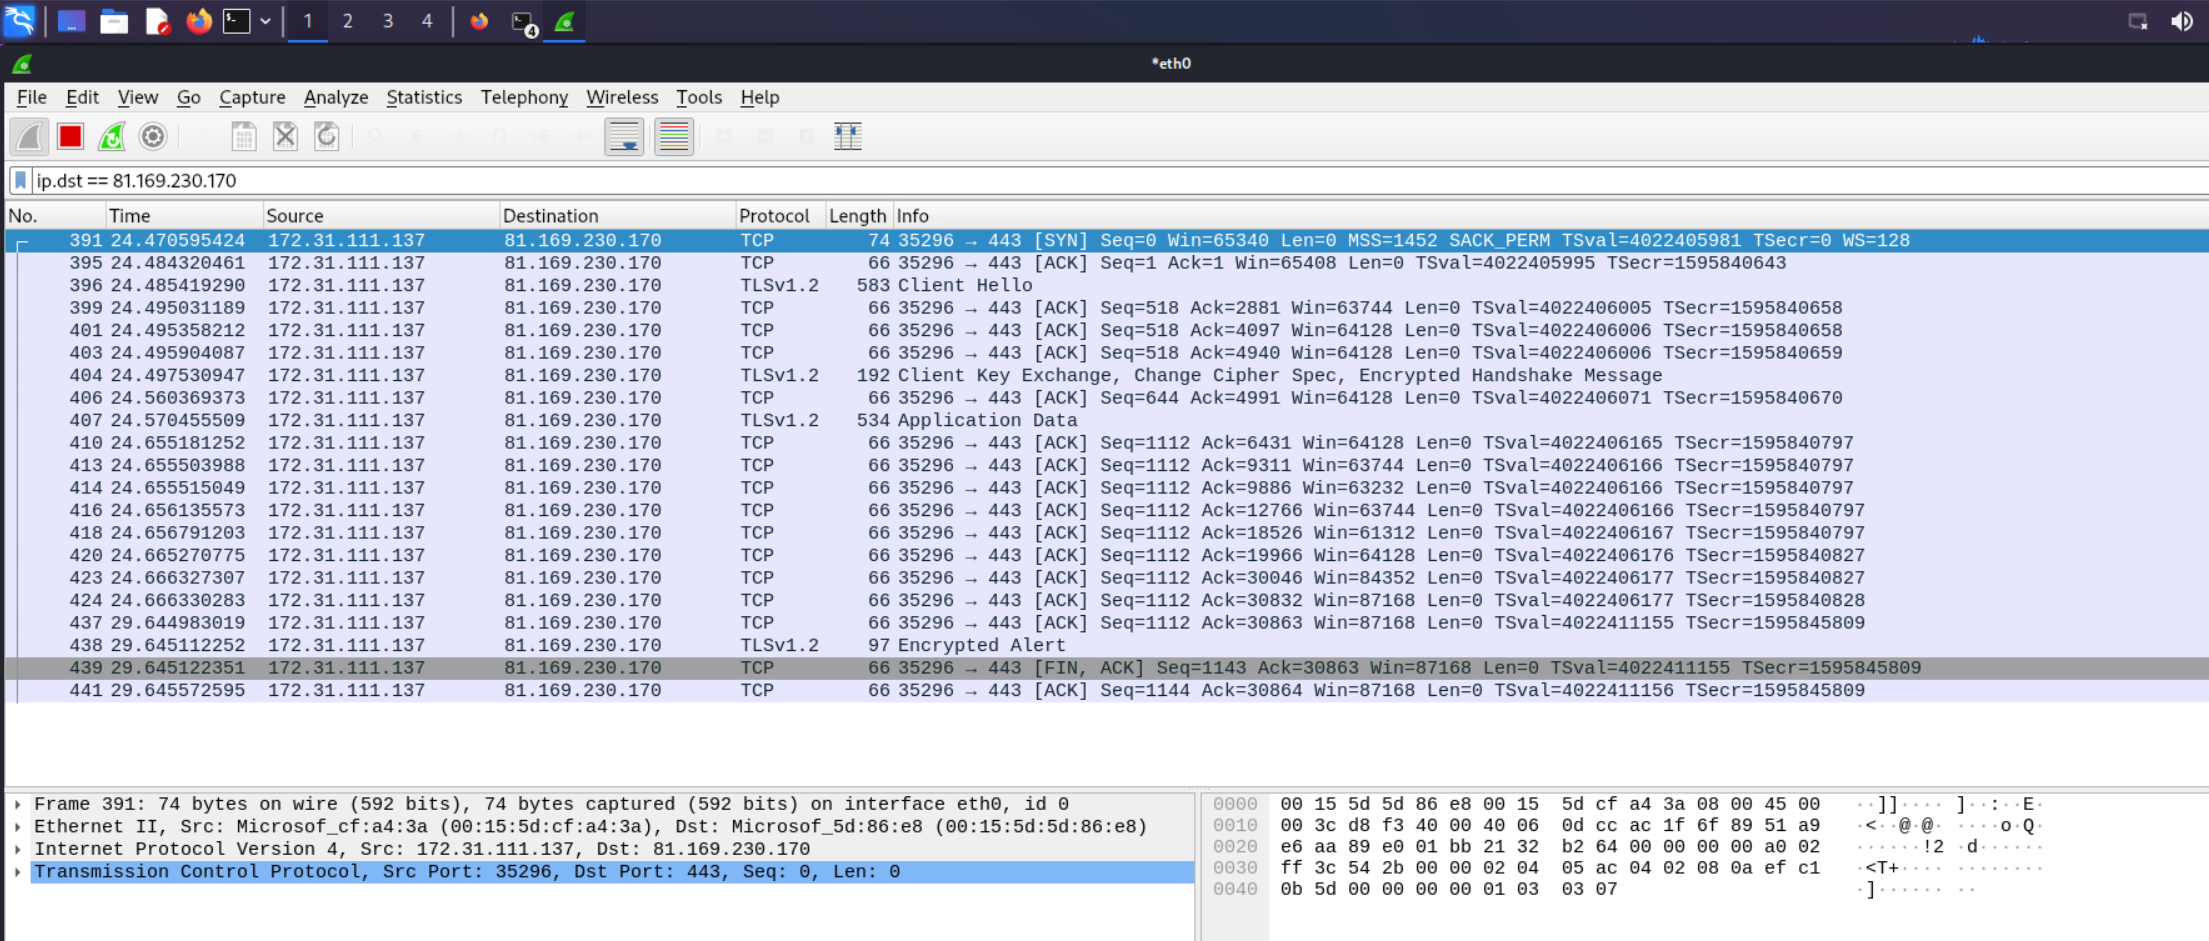
\includegraphics[width=0.75\textwidth]{images/08}
	\centering
	\caption{macspoofing: Ursprünglicher Netzwerk-Verkehr}
\end{figure}

\begin{figure}[H]
	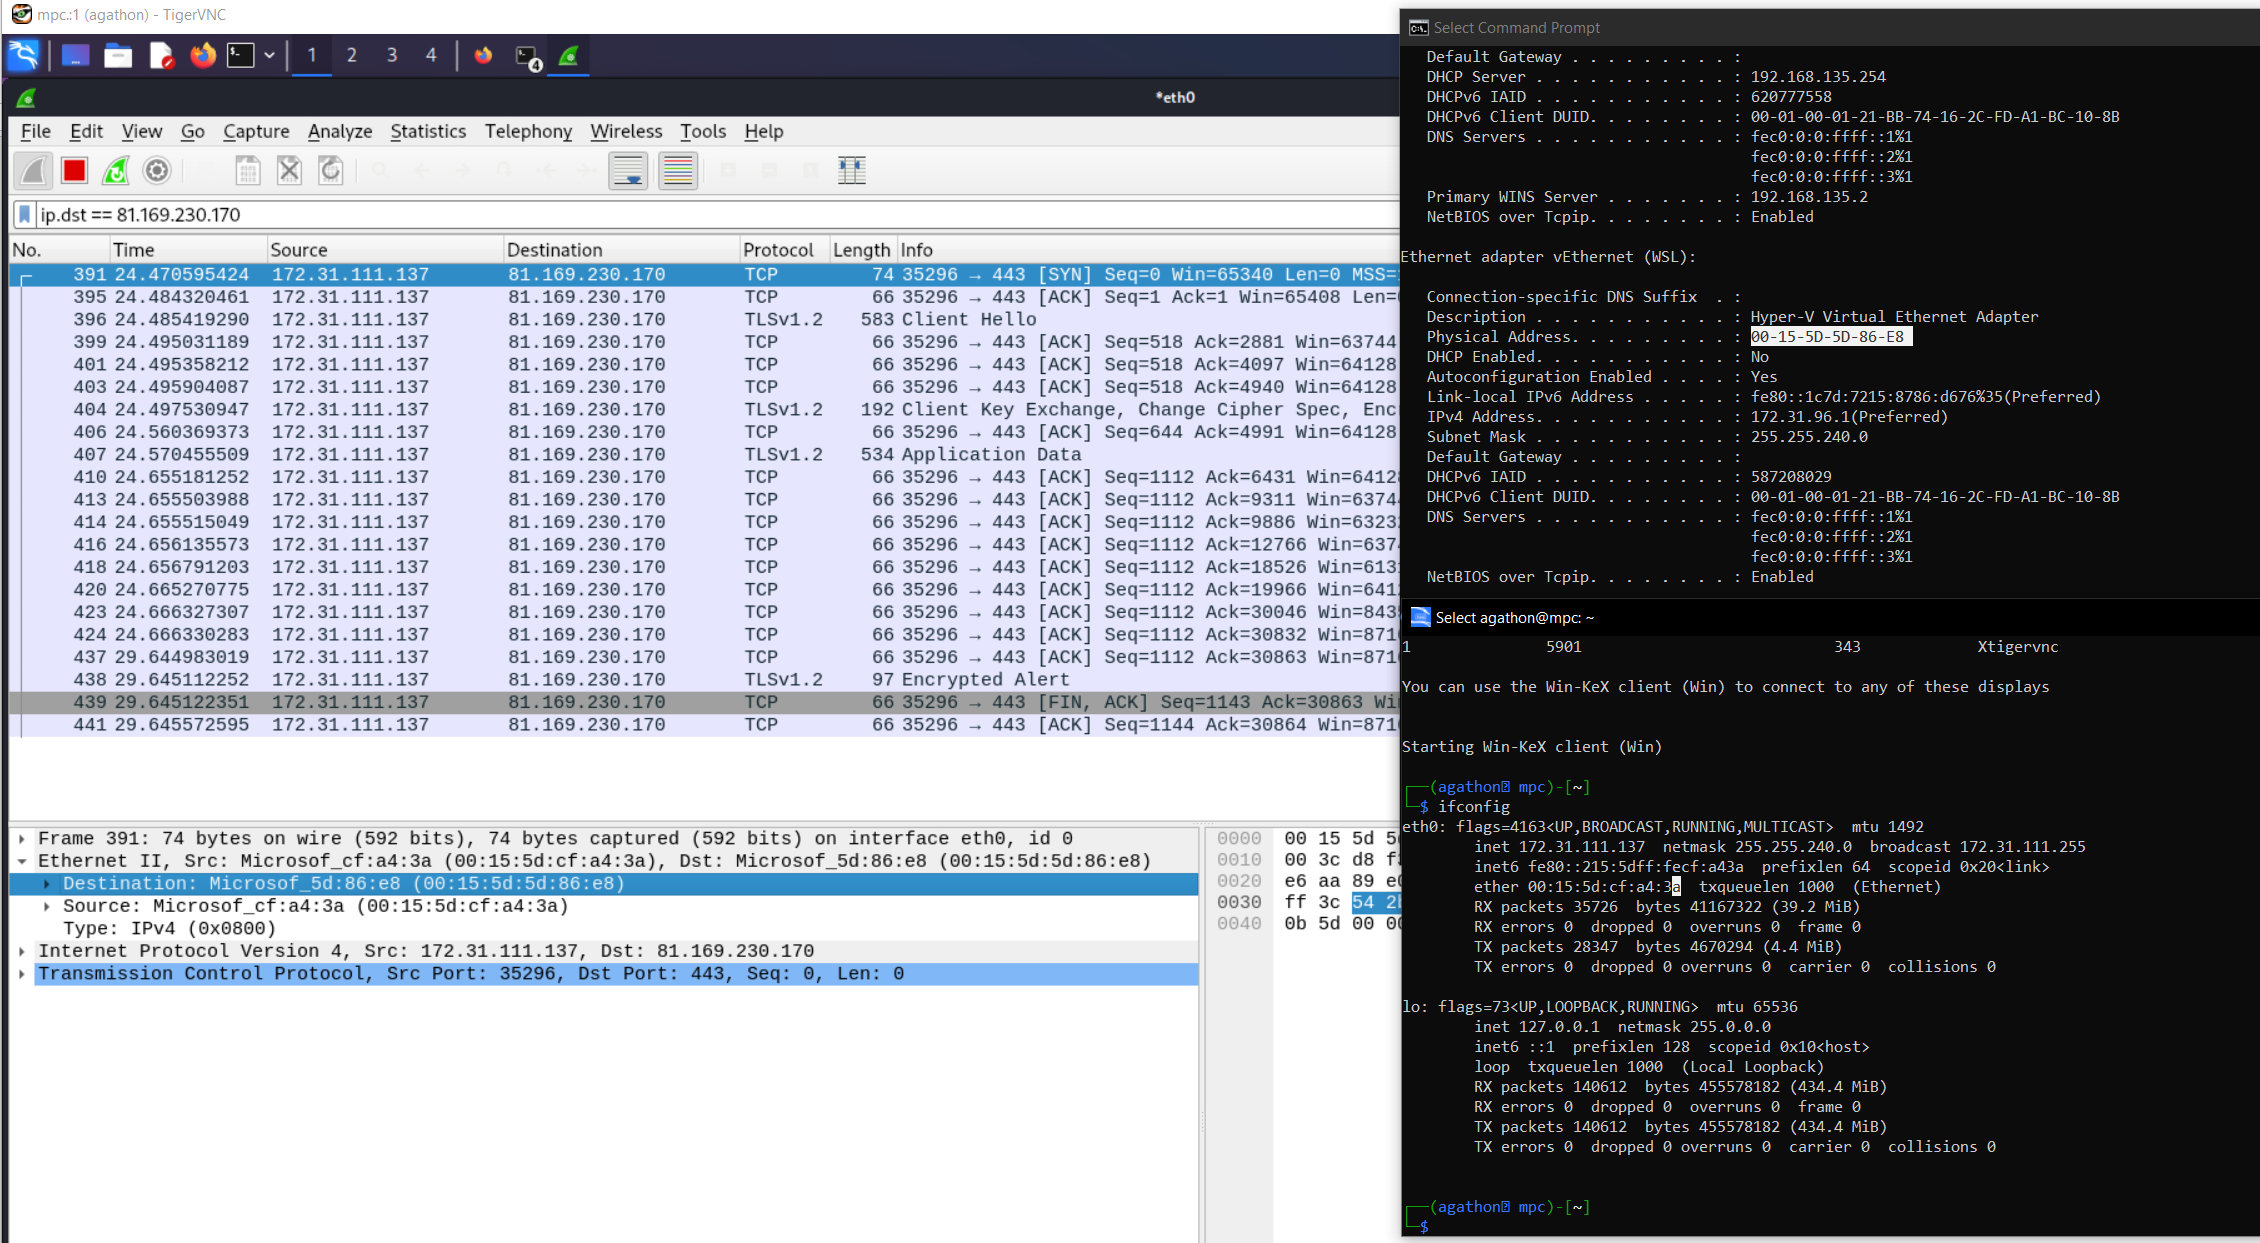
\includegraphics[width=0.75\textwidth]{images/09}
	\centering
	\caption{macspoofing: Ursprüngliche Source und Destination}
\end{figure}

In den beiden Screenshots ist zu erkennen, dass die momentane MAC-Adresse 
\texttt{XX:XX:XX} entspricht.

Nun muss zu erst das \texttt{eth0} Interface mittels \texttt{ifconfig} deaktiviert werden. 
Anschließend kann die MAC-Adresse mittels \texttt{macchanger} geändert werden. In diesem 
Beispiel haben wir lediglich die XYZ-Nummer von XYZ zu XYZ geändert und die Vendor-ID 
belassen, da eine Änderung dieser zu Problemen mit den Treibern führen kann.
Anschließend muss das Netzwerk-Interface erneut durch \texttt{ifconfig} gestartet werden.
(Siehe Abb. X-Y)

\begin{figure}[H]
	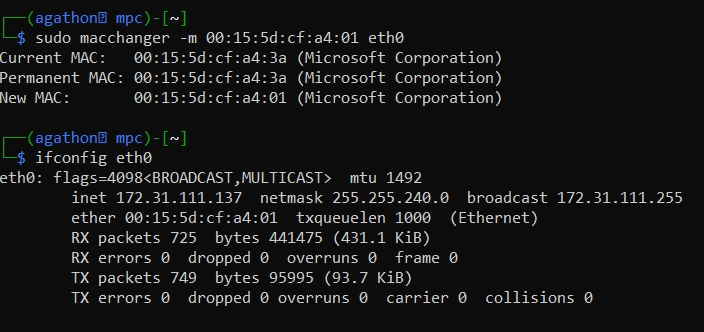
\includegraphics[width=0.75\textwidth]{images/10}
	\centering
	\caption{macspoofing: Änderung der MAC-Adresse von eth0}
\end{figure}

Bei erneuter Aufzeichnung des Traffics zum Zielserver lässt sich nun die gerade geänderte 
MAC-Adresse in dem Ethernet-Header jedes Pakets wiederfinden. (Siehe Abb. Z)

\begin{figure}[H]
	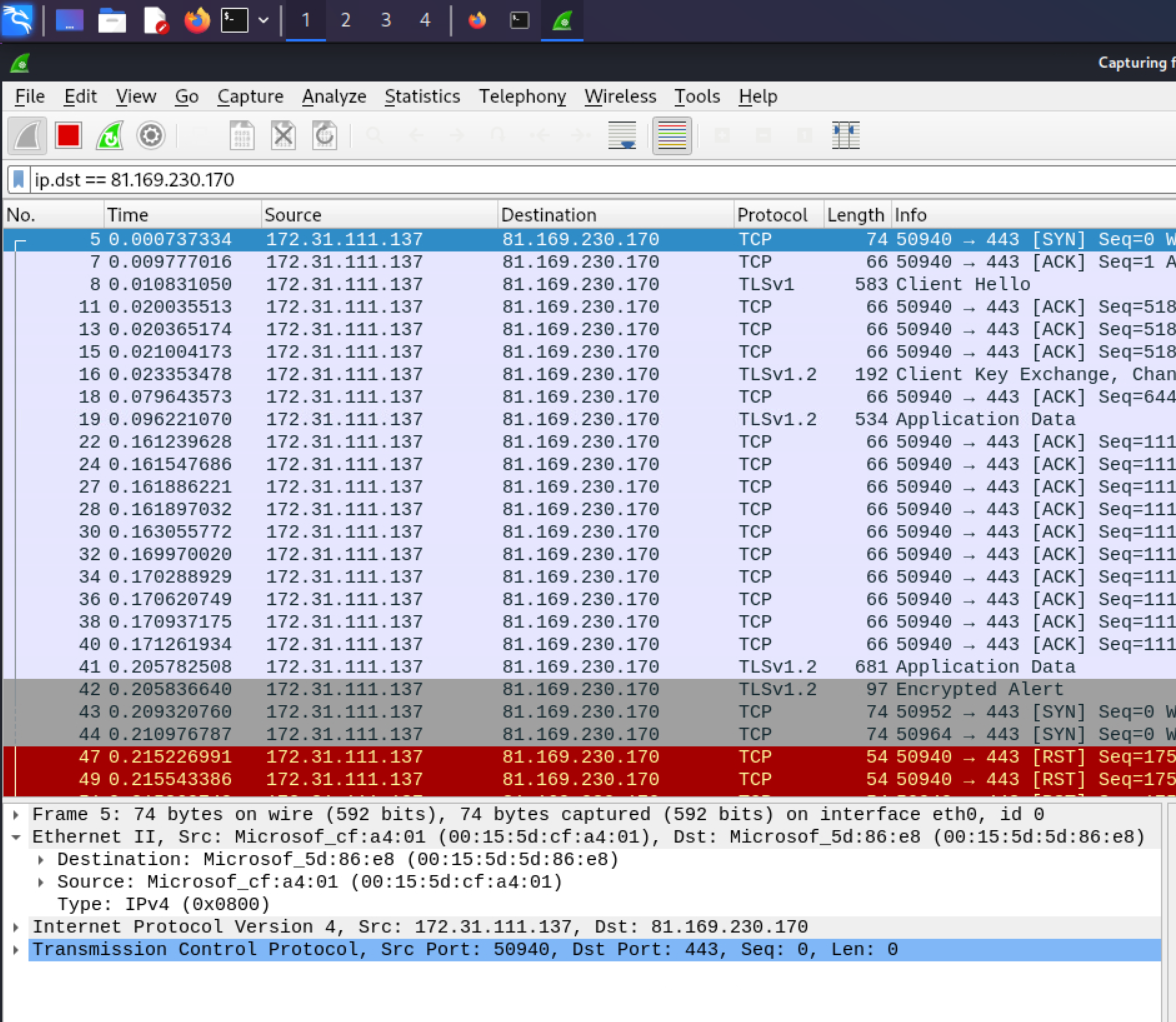
\includegraphics[width=0.75\textwidth]{images/11}
	\centering
	\caption{macspoofing: Veränderter Netzwerk-Verkehr}
\end{figure}

\newpage

\subsection{Schwachstellenscan II}

\subsubsection*{Aufgabenstellung}

Verwenden Sie das bei ParrotOS und Kali Linux vorinstallierte WPScan  (WordPress 
Vulnerability Scanner) und führen Sie einen Scan von https://nwsmooc.mooin.org durch. 
Erklären Sie die Ergebnisse.  

\begin{flushleft}
	Hinweise:	
\end{flushleft}


\begin{itemize}
	\item Es ist keine Registrierung beim Anbieter erforderlich. Durch eine Registierung würde man ein Token erhalten, um Schwachstellentests durchführen zu können. So ist die Aufgabe auf eine Informationssammlung beschränkt.
	\item Bei einem Test mit ParrotOS gab es zunächst eine Fehlermeldung, dass ein Update der Datenbank nicht möglich sei. Ein allgemeines Update
		(\texttt{sudo apt-get update \&\& apt-get upgrade}) konnte dieses Problem beseitigen.
\end{itemize}

Sollten Sie Mac oder Linux verwenden, dann installieren Sie WPScan direkt von Github. 
Sollten Sie keine Möglichkeit zur Durchführung dieses Aufgabenteils finden, sprechen 
Sie die Betreuenden auf eine Ersatzaufgabe an.

\subsubsection*{Antwort}

Der Aufgabe entsprechend haben wir einen Schwachstellen-Scan bei dem vorgegebenen 
Zielserver durchgeführt. Dieser hat das folgende Ergebnis erzielt:

\begin{figure}[H]
	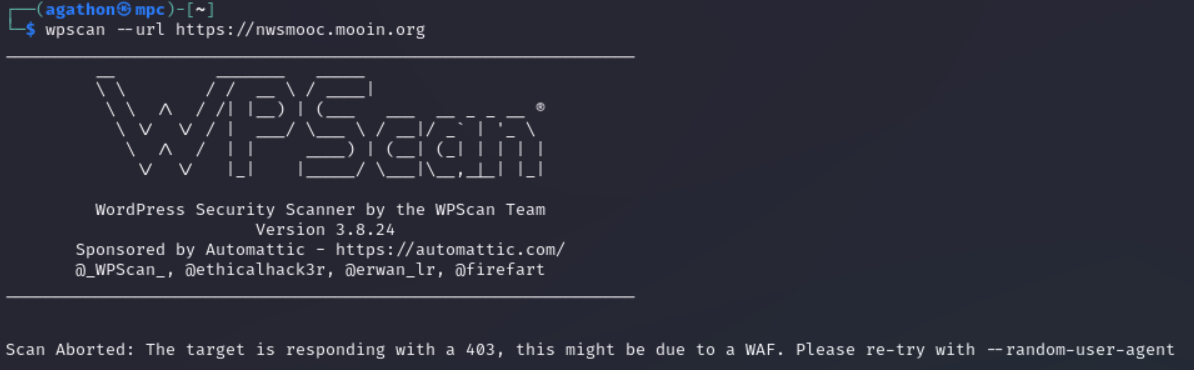
\includegraphics[width=0.75\textwidth]{images/12}
	\centering
	\caption{wpscan: Fehler}
\end{figure}

Nun musste die flag angehängt werden

\begin{figure}[H]
	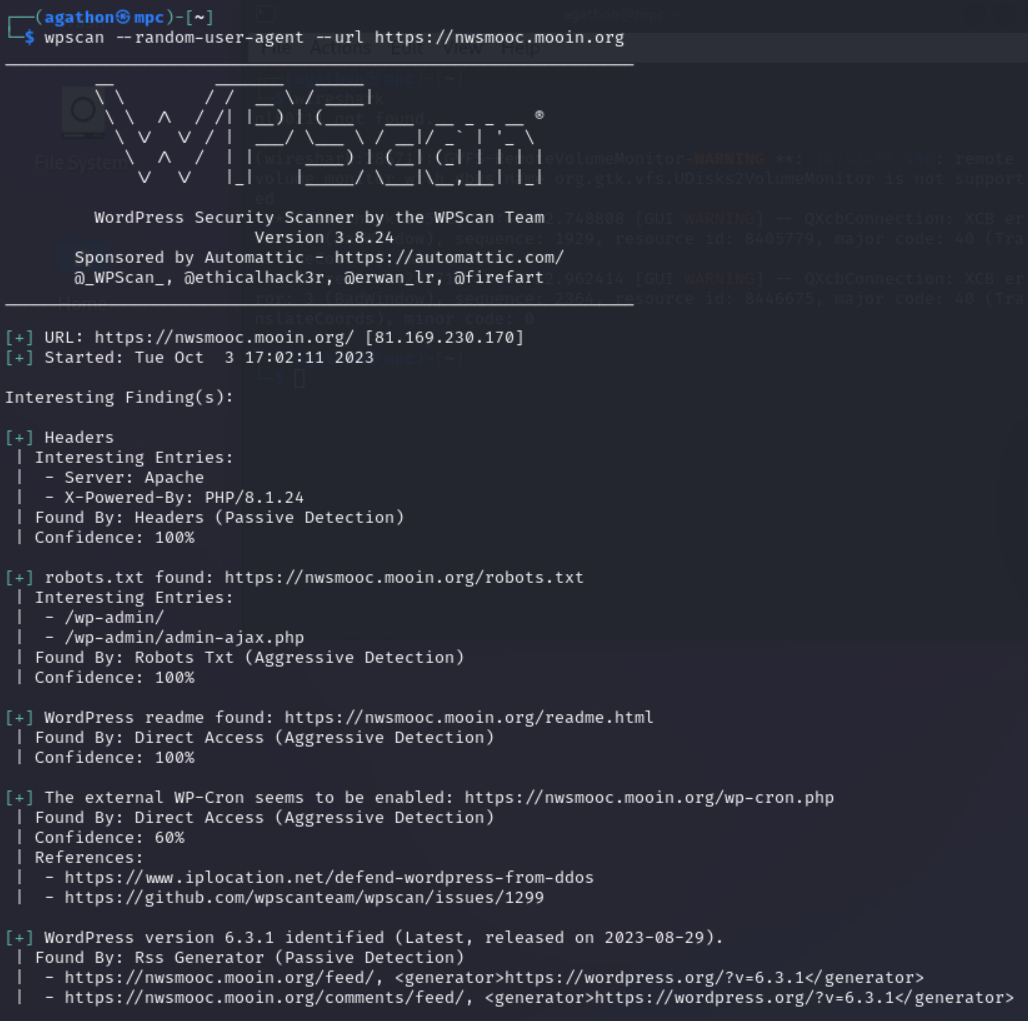
\includegraphics[width=0.75\textwidth]{images/13}
	\centering
	\caption{wpscan: Ergebnis 1/2}
\end{figure}

\begin{figure}[H]
	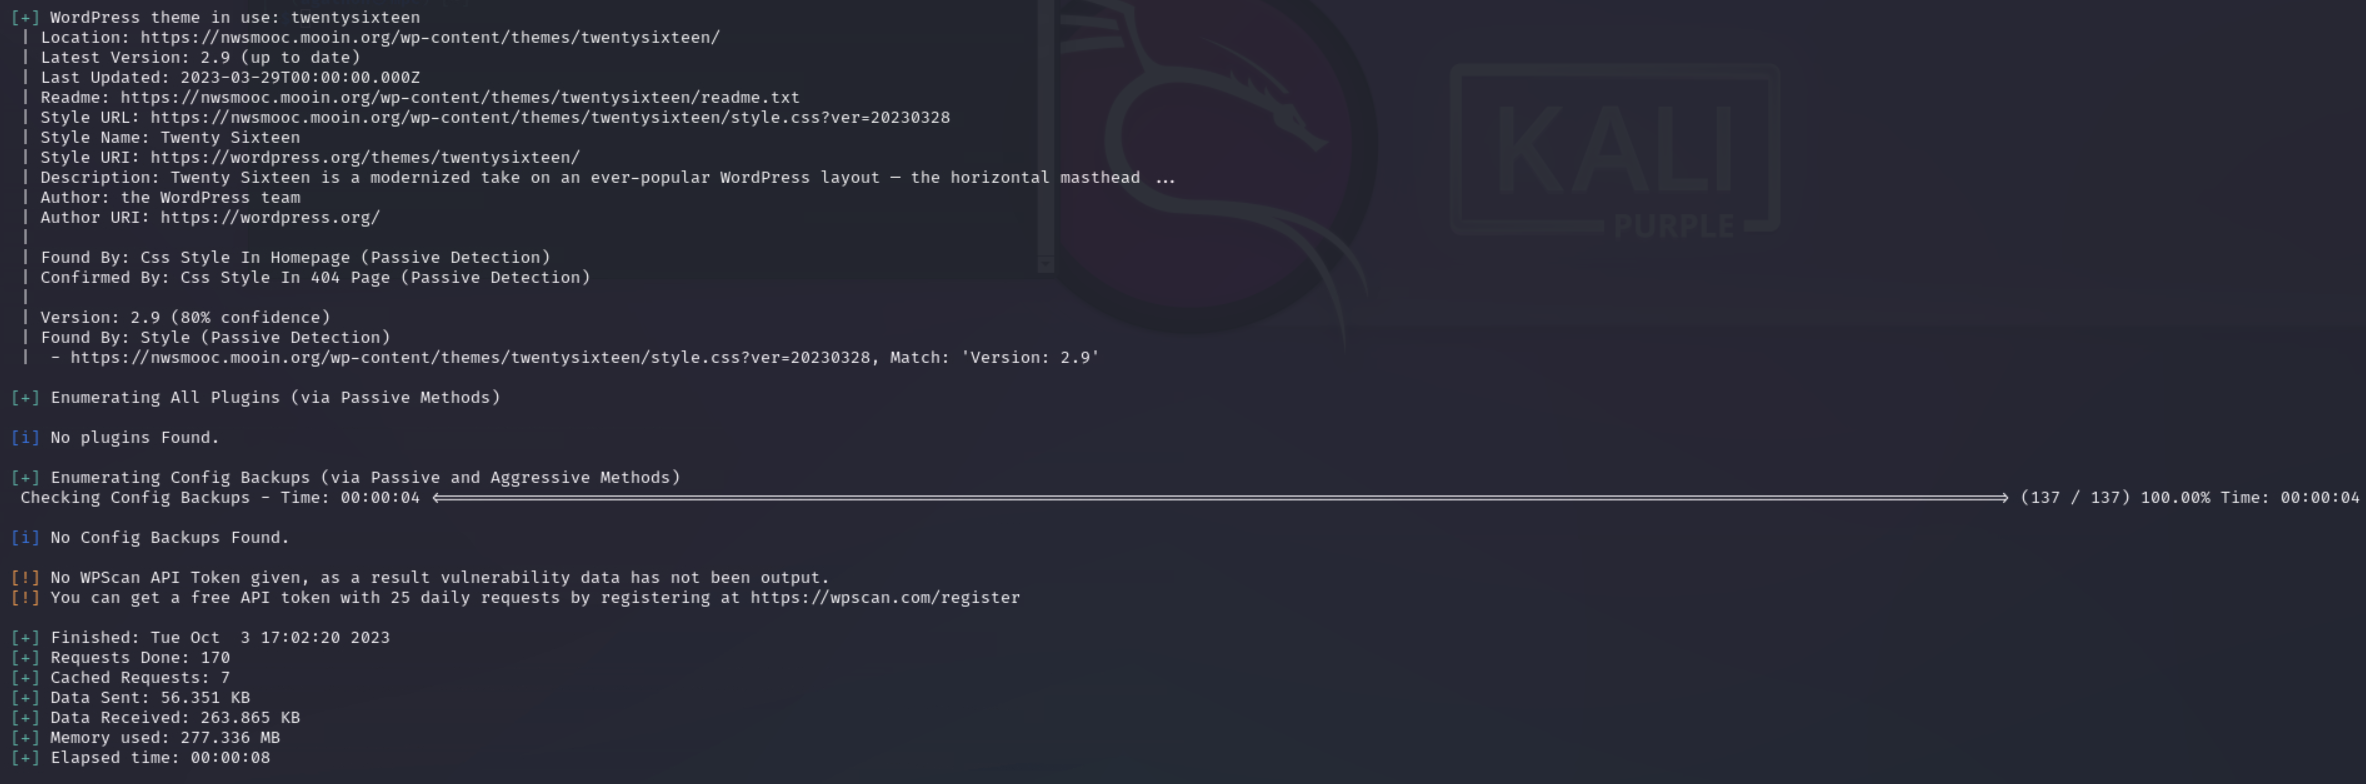
\includegraphics[width=0.75\textwidth]{images/14}
	\centering
	\caption{wpscan: Ergebnis 2/2}
\end{figure}

Hieraus lassen sich folgende Informationen ableiten: XYZ

\newpage

\subsection{Google-Hacking}

\subsubsection*{Aufgabenstellung}

Mit "Google Hacking" ist gemeint, dass man die Google Suche zum Auffinden von
Softwareinstallationen mit Schwachstellen nutzen kann. Eine Sammlung von Beispielen ist 
bei \url{https://www.exploit-db.com/google-hacking-database/} zu finden. Erklären Sie 
anhand von drei selbstgewählten Beispielen, was man damit herausfinden kann.
Achtung: Firefox und Google Chrome warnten teilweise beim Aufruf der Seite und bezeichneten diese als riskant. Man kann die Seite aber aus einem Browser innerhalb von Kali Linux oder ParrotOS aufrufen, dann kommt keine Warnung.

\subsubsection*{Antwort}

Innerhalb der Exploit-Datenbank haben wir uns drei, unserer Meinung nach, besonders 
interessante Beispiele ausgesucht.



Das erste unserer Beispiele beruht auf dem Prinzip Google-Filter zu verwenden um von 
Google indexierte Dateien mit bestimmten Namen oder Dateiendungen zu finden. So können zum 
Beispiel falsch konfigurierte Web-Server aus Versehen vertrauliche Daten öffentlich 
zugänglich machen. Ein interessantes Beispiel ist hierbei nach rohen SQL-Backups zu 
suchen. Diese könnten, bei schlechten Sicherheitsmaßnahmen des Servers, rohe Nutzerdaten 
enthalten und somit entweder einen Angriff auf die betroffenen Accounts ermöglichen oder 
weiter verwendet werden um Zugriff auf andere, möglicherweise interessantere, Systeme zu 
erlangen.


\begin{figure}[H]
	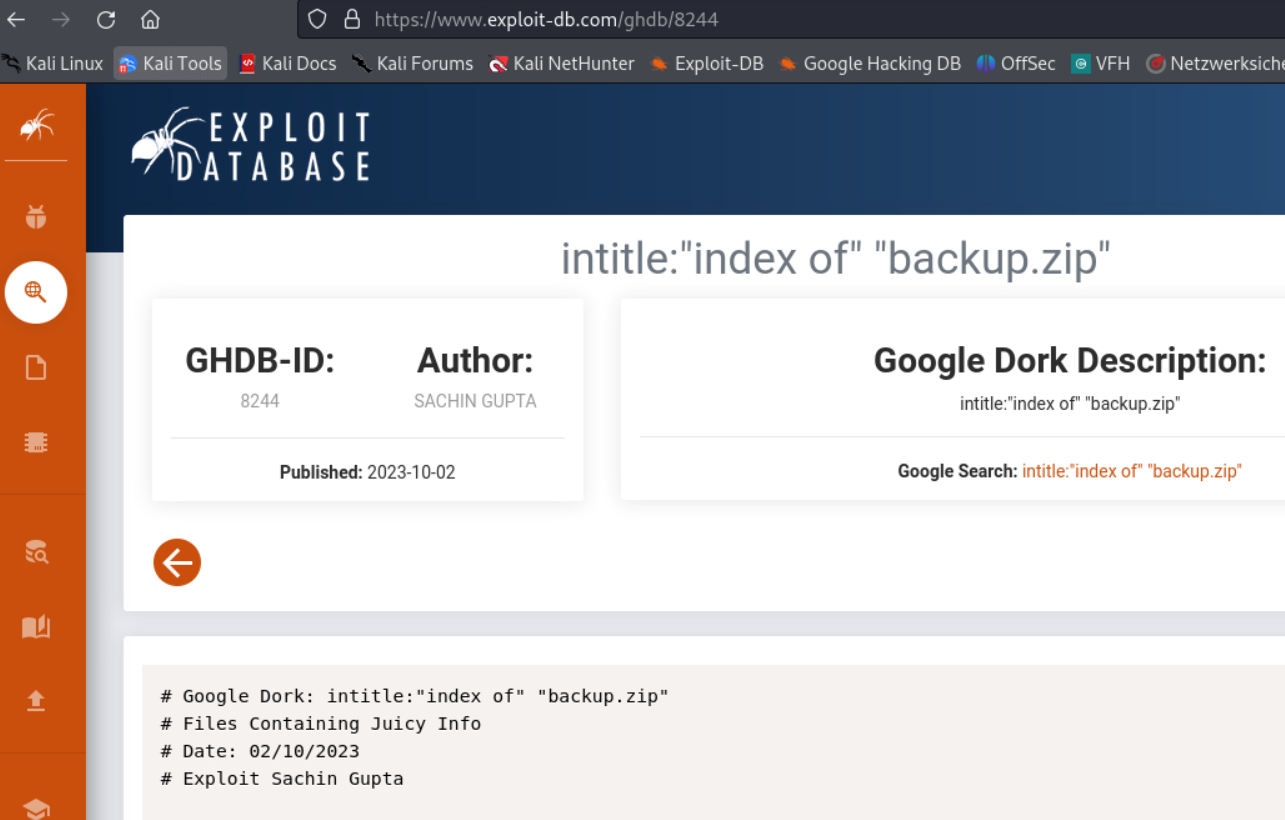
\includegraphics[width=0.75\textwidth]{images/15}
	\centering
	\caption{Google Hacking: Backup: Schwachstelle}
\end{figure}

\begin{figure}[H]
	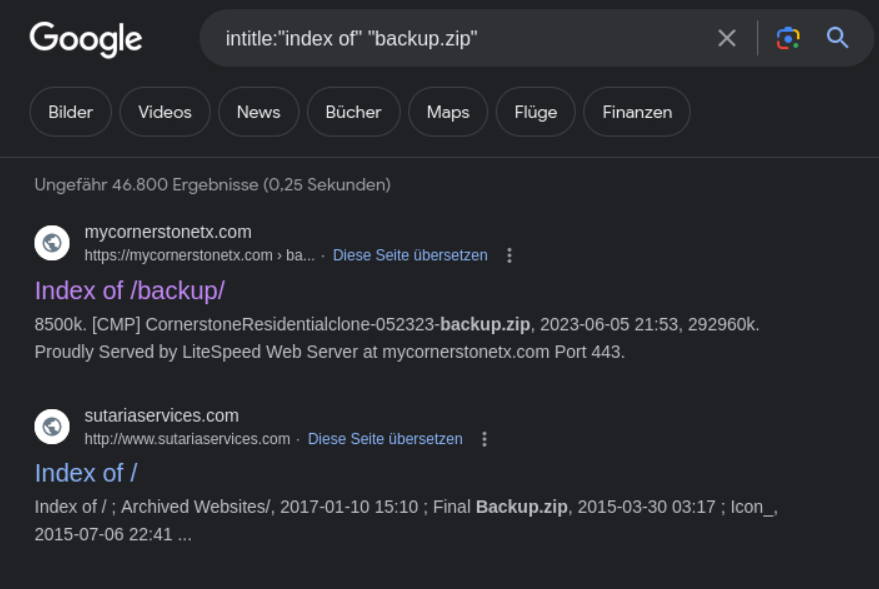
\includegraphics[width=0.75\textwidth]{images/16}
	\centering
	\caption{Google Hacking: Backup: Google Suche}
\end{figure}

\begin{figure}[H]
	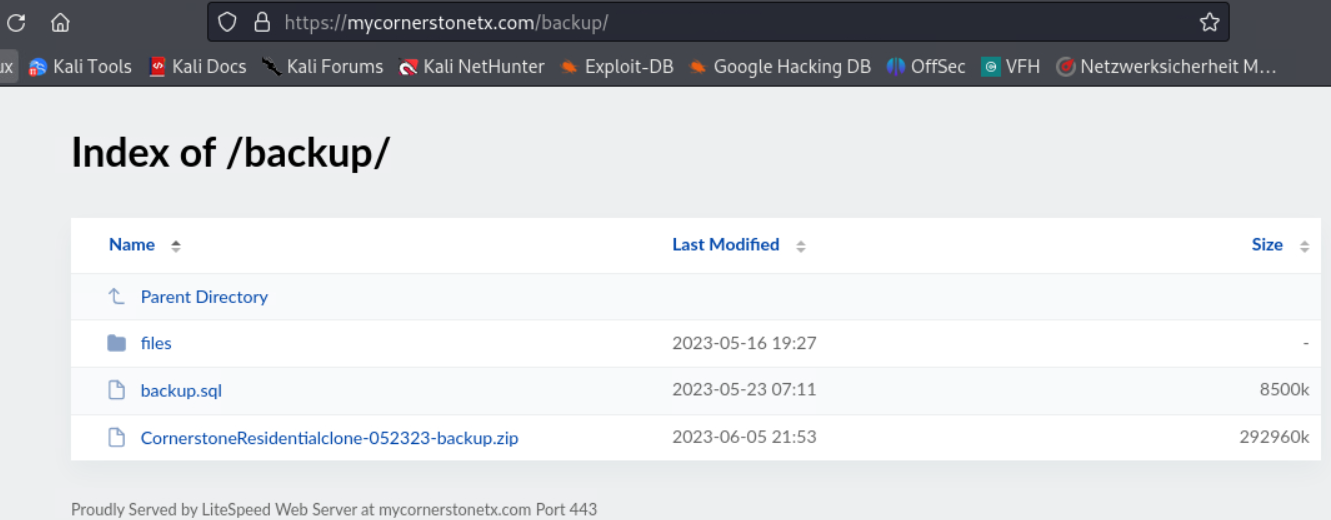
\includegraphics[width=0.75\textwidth]{images/17}
	\centering
	\caption{Google Hacking: Backup: Ergebnis}
\end{figure}

Das zweite unserer Beispiele ist die Suche nach Webseiten die Tokens o.ä. vertraulichen 
Informationen im Klartext enthalten. Dies ist ein besonders hohes Risiko bei Seiten, die 
Quellcode enthalten (Wie z.B. Pastebin oder GitHub). Das Beispiel in unserer Abbildung 
sucht nach Tokens auf öffentlich-zugänglichen Pastebin-Seiten.

\begin{figure}[H]
	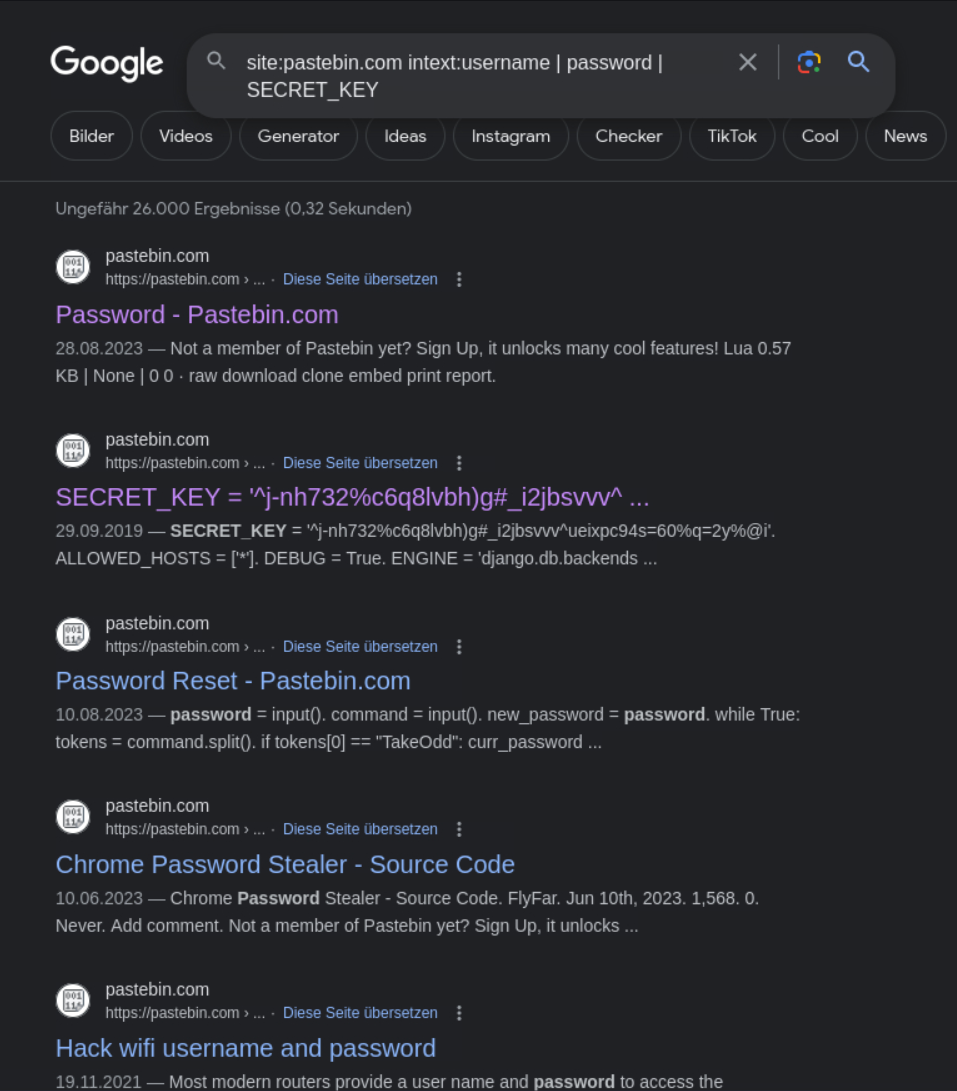
\includegraphics[width=0.75\textwidth]{images/18}
	\centering
	\caption{Google Hacking: Tokens: Suche}
\end{figure}


\begin{figure}[H]
	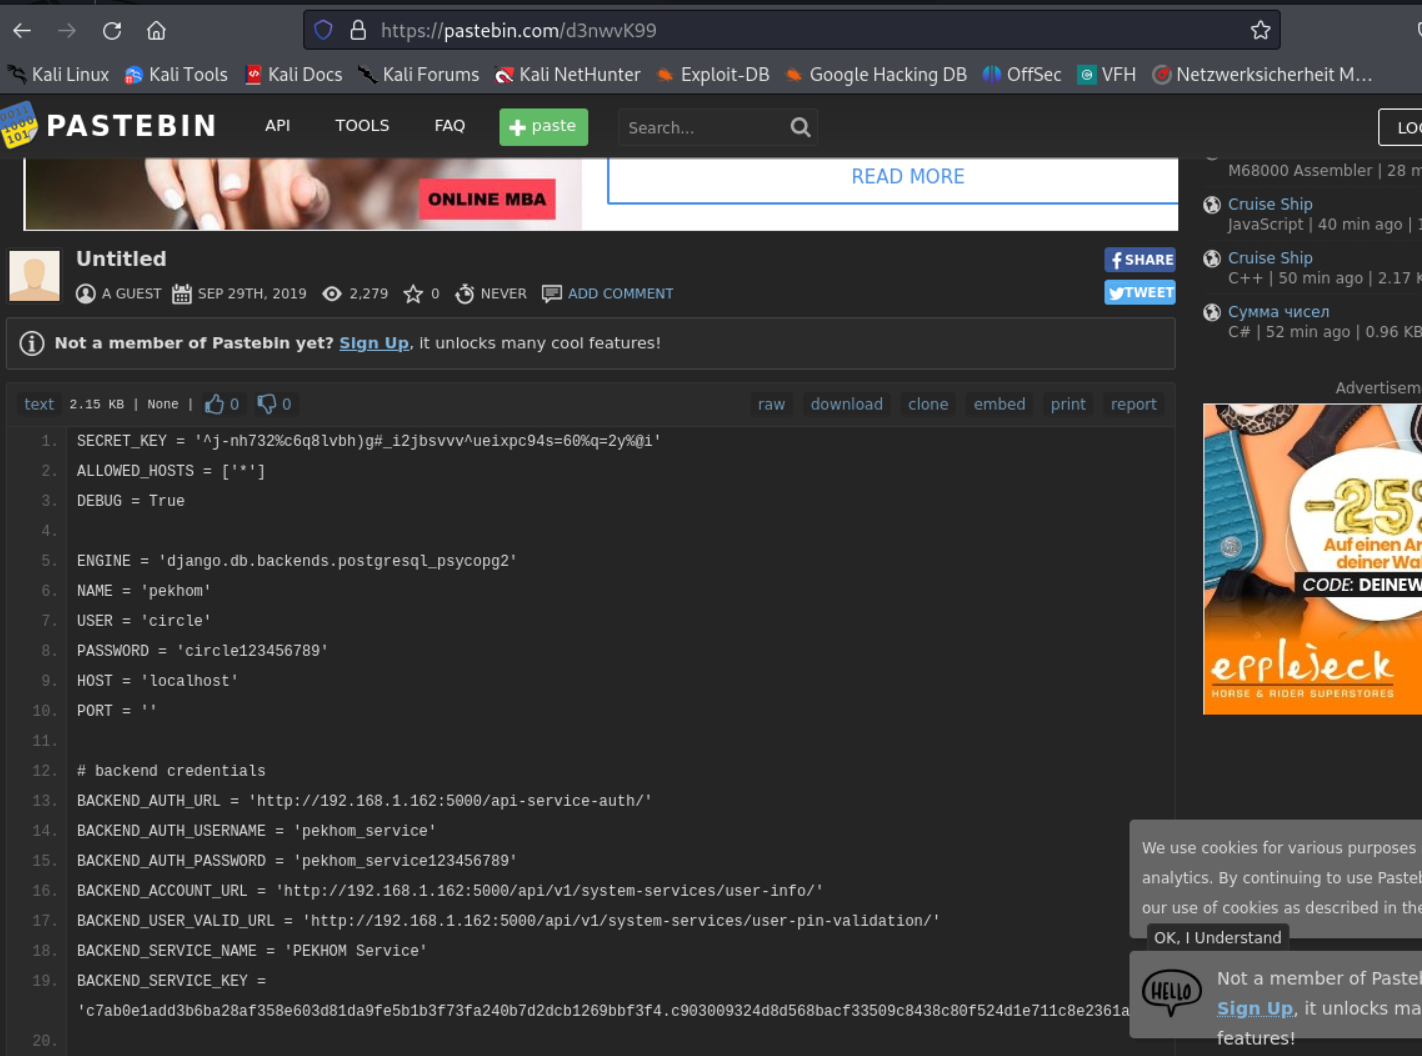
\includegraphics[width=0.75\textwidth]{images/19}
	\centering
	\caption{Google Hacking: Tokens: Ergebnis}
\end{figure}

Die letzte, und wohl kritischte, Schwachstelle, die wir im Rahmen dieser Aufgabe gefunden 
haben,


\begin{figure}[H]
	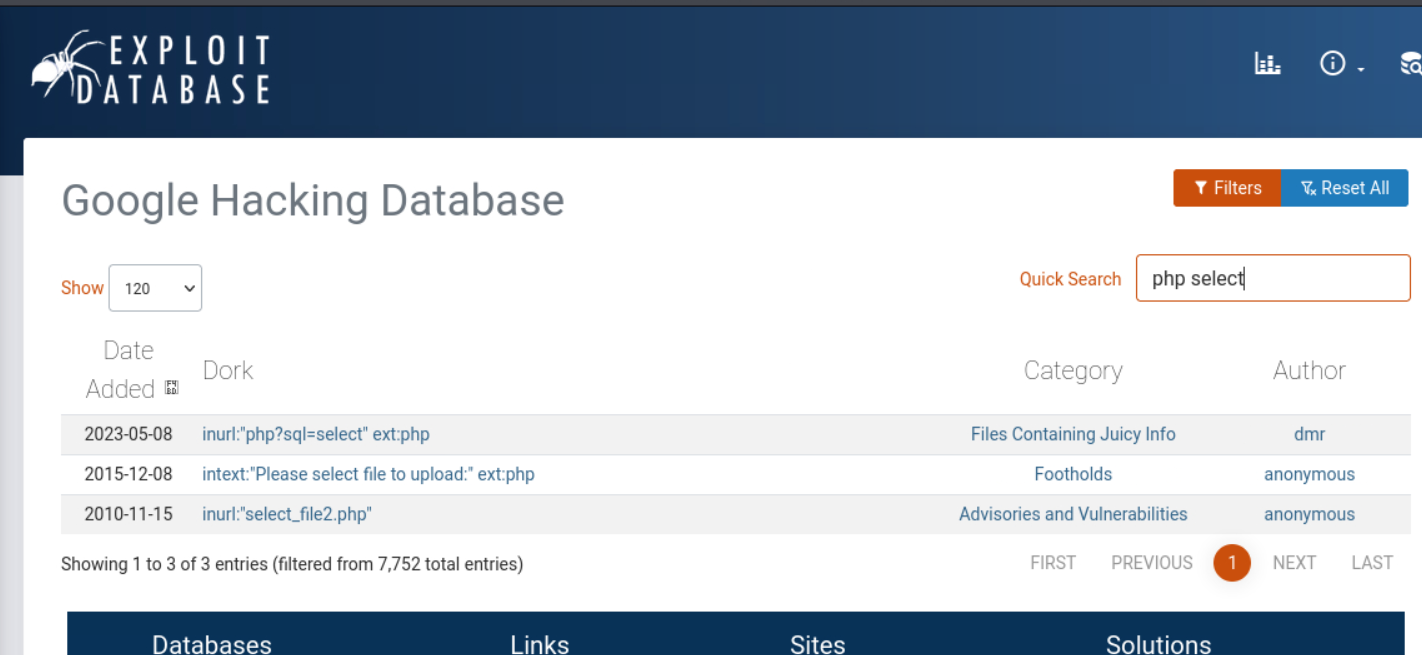
\includegraphics[width=0.75\textwidth]{images/20}
	\centering
	\caption{Google Hacking: SQL Injektion: Schwachstelle}
\end{figure}

\begin{figure}[H]
	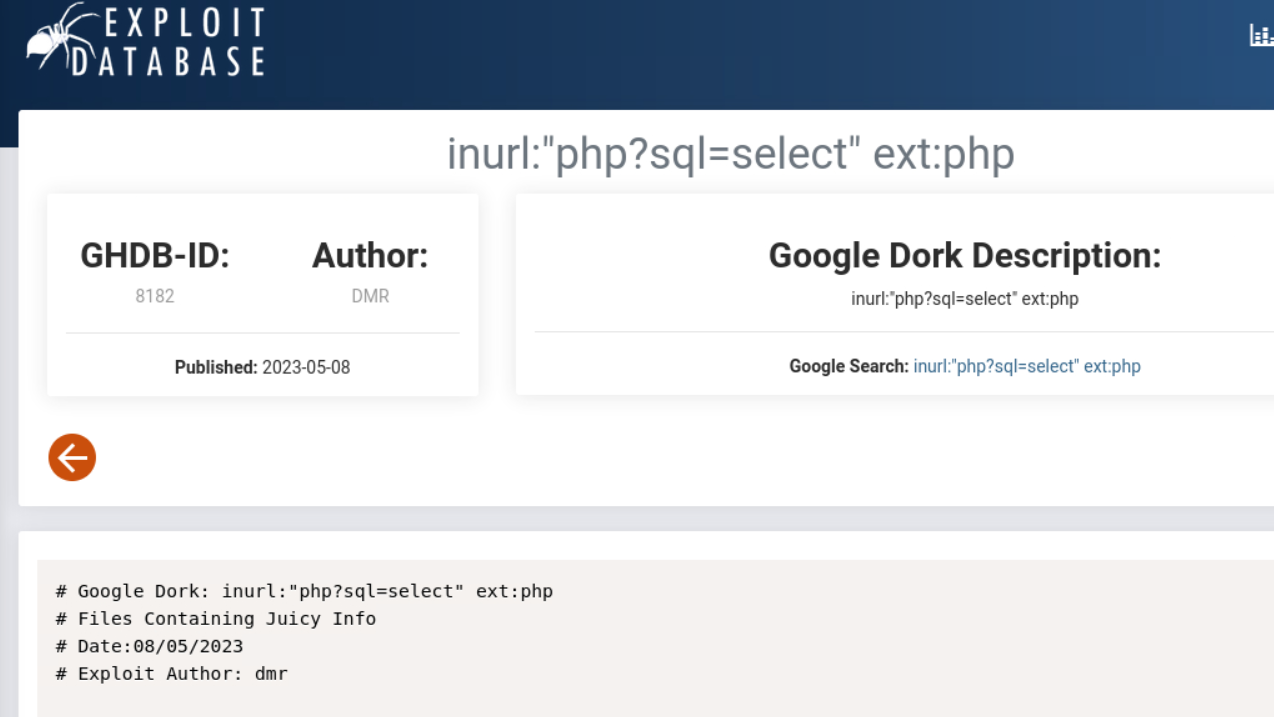
\includegraphics[width=0.75\textwidth]{images/21}
	\centering
	\caption{Google Hacking: SQL Injektion: Schwachstelle}
\end{figure}

\begin{figure}[H]
	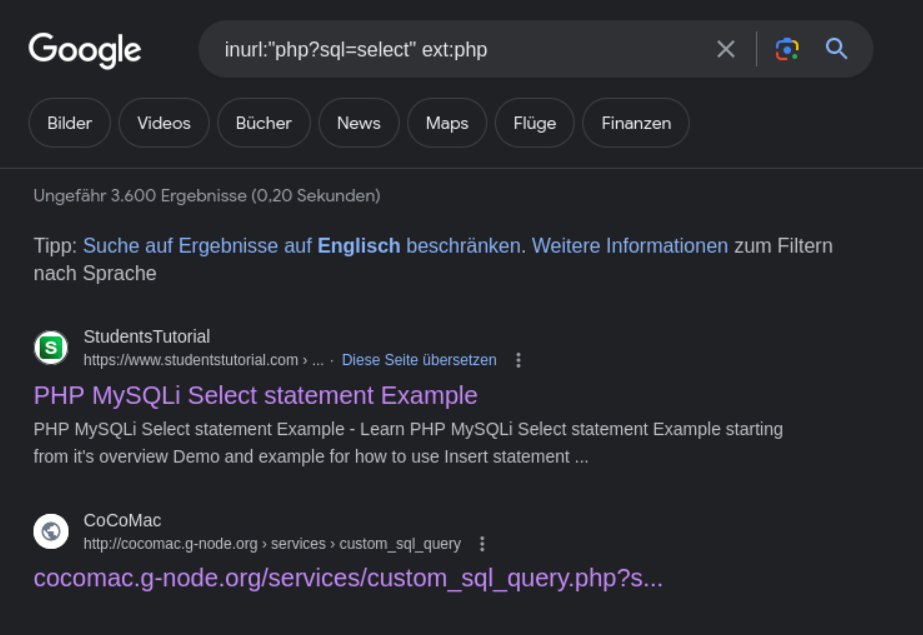
\includegraphics[width=0.75\textwidth]{images/22}
	\centering
	\caption{Google Hacking: SQL Injektion: Suche}
\end{figure}


\begin{figure}[H]
	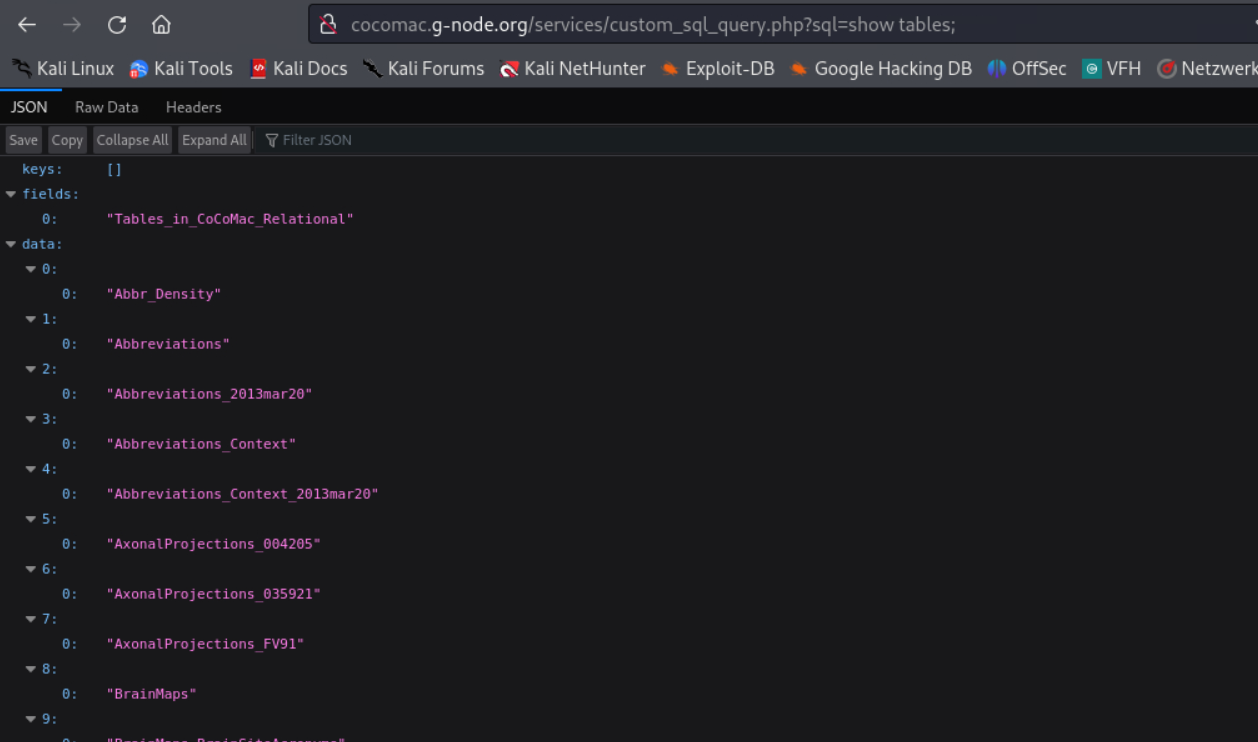
\includegraphics[width=0.75\textwidth]{images/23}
	\centering
	\caption{Google Hacking: SQL Injektion: Ergebnis}
\end{figure}


\end{document}
